\section{Methods}
\subsection{Neural network}
The first model is a model from the one of the exercise sessions about multiclass-classificication neural networks. The architecture of the model is a feedforward neural network with multiple densely connected layers. Each layer contains of a number of neurons which are decreasing progressively. The output layer has a number of neurons equal to the number of classes.

The learning in this model is done through backpropagation. This involves iteratively adjusting the weights of the connections based on the error of the prediction. The objective is to find the optimal weights that minimize the cross-entropy loss between the predicted probabilities and the true class labels. Because of timing issues, the training of the first model is done on a smaller set of 50 of the 525 classes. 

The first model was the model of the exercise session with 3 layers. In these layers the amount of neurons was changed to confirm with the amount of classes at the output layers, and the layers above have a higher number of nodes. The basic neural network model consist of two layers of 64 neurons and one layer of 50 neurons according to the figure \ref{fig:NN with 3 layers}. The improved neural network has 8 layers going down from 1024 neurons to 50 neurons, according to the figure \ref{fig:NN with 8 layers}

The basic neural network model is a model consisisting of a input layer which takes in the data type being (32, 32, 3) because the images are decreased in quality to improve the training. All the connected layers different from the output layer are fully connected layers with RELU activation,  this introduces non-linearity into the neural network. This activation makes the computation more efficient because it just involves a simple threshold at 0, which is way less computational hard then other activation systems. It is given by the following formula:

\[
\text{ReLU}(x) = \begin{cases}
    x & \text{if } x > 0 \\
    0 & \text{if } x \leq 0
\end{cases}
\]

The activation in the output layer is softmax, this transforms a vector of numbers into a probability distribution. It makes sure that the output values are between 0 and 1 and it sums to 1, this makes it possible for representing the probabilities. It is used together with cross-entropy loss. It measures the difference between the predicted probabilities and the true distribution of the labels. It is given by the following formula: 

\[\text{softmax}(\mathbf{x})_i = \frac{e^{x_i}}{\sum_{j=1}^{N} e^{x_j}}\]

Both of those neural network models are trained with a learning rate of 0.001. This value determines the stepsize at each iteration, while moving towards a minimum of the loss function. If the learning rate is big this can lead to an overshooting of the minimum and a failure to converge. When the learning rate is too small the convergence will happen really slowly. 

\begin{figure}[h]
    \centering
    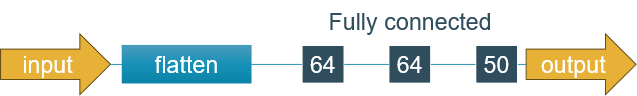
\includegraphics[width=0.5\textwidth]{figs/basic nn.png}
    \caption{NN with 3 connected layers architecture}
    \label{fig:NN with 3 layers}
\end{figure}

\begin{figure}[h]
    \centering
    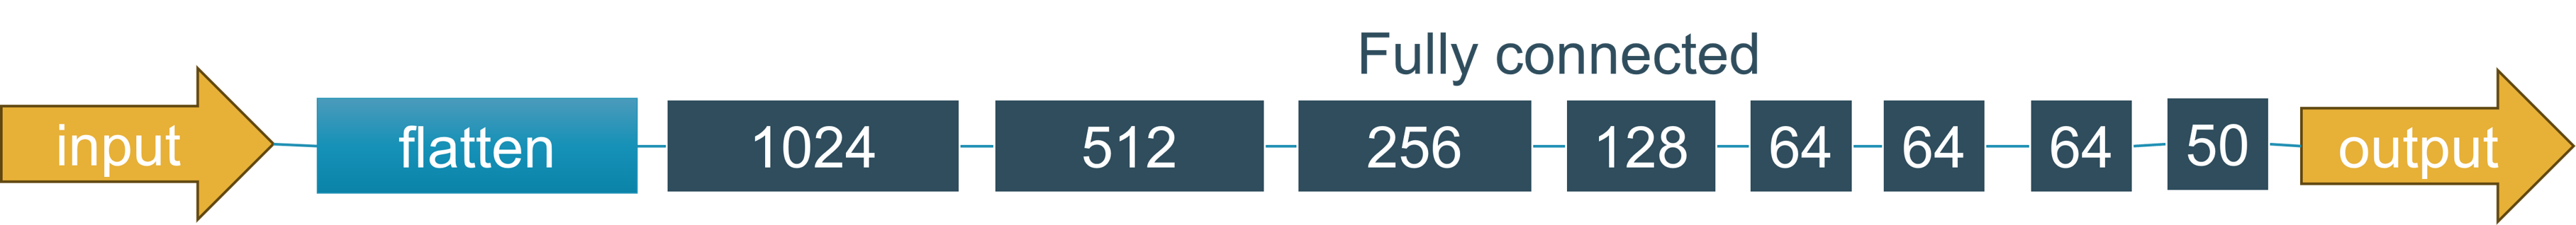
\includegraphics[width=0.5\textwidth]{figs/improved NN.png}
    \caption{NN with 8 connected layers architecture}
    \label{fig:NN with 8 layers}
\end{figure}

\subsection{ResNet}
ResNet, short for Residual Network, is a type of neural network architecture that was designed to enable the training of much deeper networks than was previously feasible. Introduced by Microsoft researchers in 2015, ResNet quickly became famous for its effectiveness, especially in image classification tasks. \citet{he_deep_2016} The ResNet architecture is composed of a series of residual blocks, which are composed of a series of convolutional layers. 

\begin{figure}[h]
    \centering
    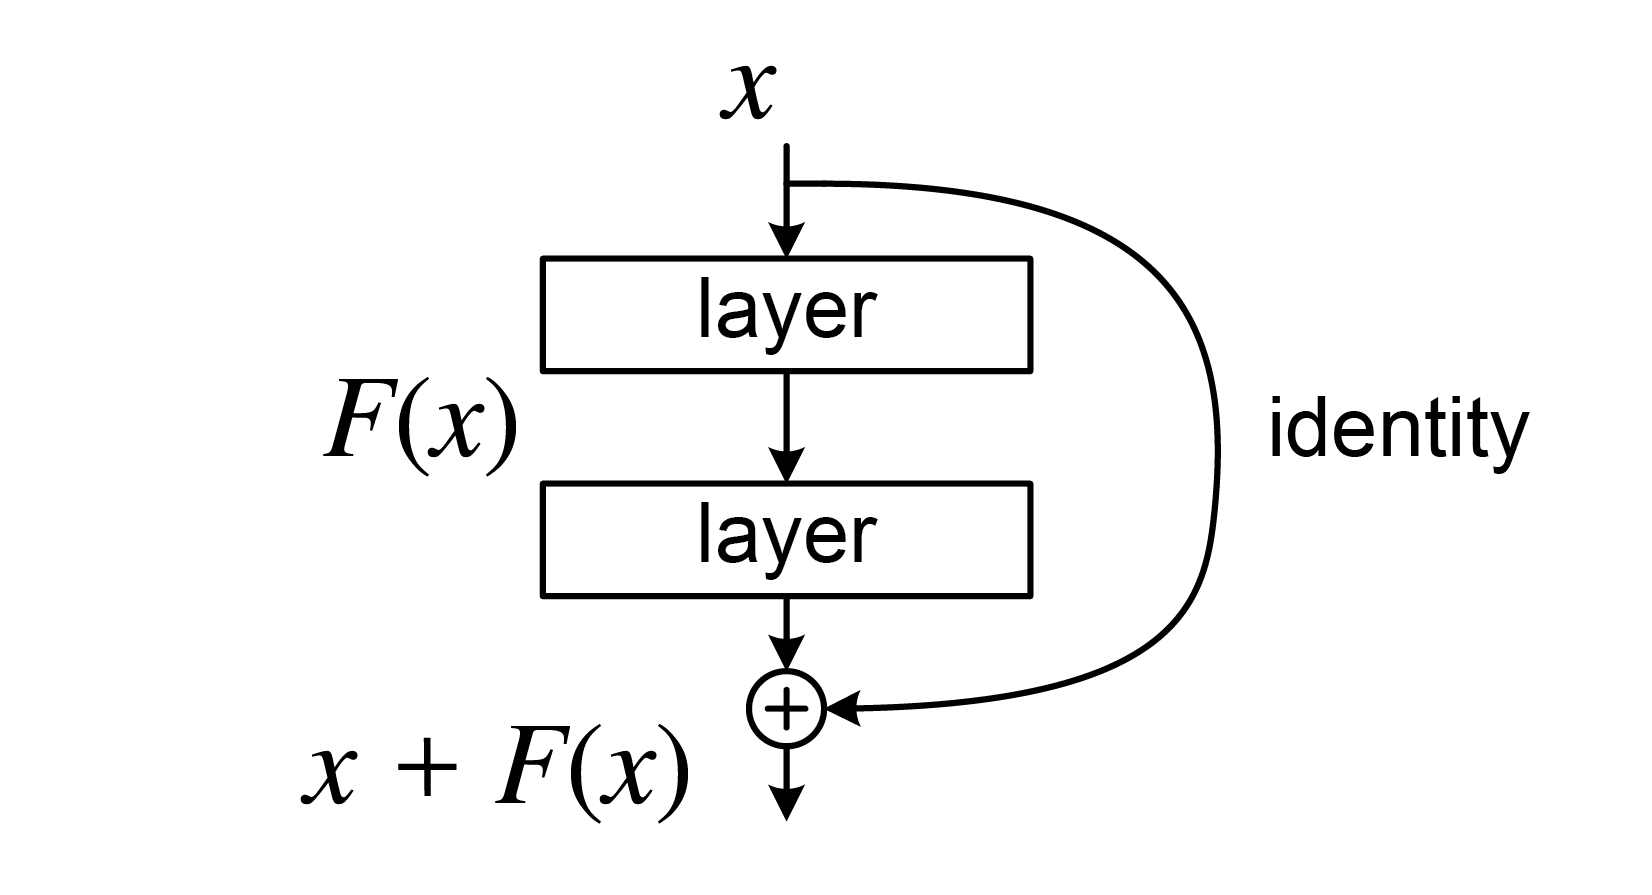
\includegraphics[width=0.5\textwidth]{figs/ResBlock.png}
    \caption{ResNet architecture}
    \label{fig:resnet}
\end{figure}

The ResNet (Residual Network) architecture, as illustrated in Figure \ref{fig:resnet}, represents a significant advancement in deep neural networks. This architecture is primarily characterized by its residual blocks and skip connections. The structure of ResNet can be described as follows:

\begin{itemize}
    \item \textbf{Residual Blocks:} Each residual block in ResNet is composed of several convolutional layers. These layers are designed to learn the residual functions with reference to the layer inputs. A typical residual block contains two or three convolutional layers.

    \item \textbf{Convolutional Layers:} Within each residual block, convolutional layers are used for feature extraction. Each layer applies a set of learnable filters to the input. The convolutional layers in ResNet typically use batch normalization and a ReLU activation function.

    \item \textbf{Skip Connections:} A distinctive feature of ResNet is the use of skip connections (or shortcut connections). These connections allow the input of a residual block to be directly added to its output. Mathematically, if $\mathbf{x}$ is the input and $\mathcal{F}(\mathbf{x})$ is the output of the residual block, the final output of the block is $\mathcal{F}(\mathbf{x}) + \mathbf{x}$.

    \item \textbf{Identity Function Learning:} Skip connections facilitate the learning of the identity function. This is crucial in deeper networks as it mitigates the problem of vanishing gradients, enabling the training of very deep networks.

    \item \textbf{Depth of Network:} Thanks to skip connections, ResNet architectures can be significantly deeper than traditional convolutional neural networks. Models with various depths have been proposed, such as ResNet-50, ResNet-101, and ResNet-152, indicating the number of layers in the network.
\end{itemize}

The overall architecture of ResNet enables the training of deep neural networks with improved performance on tasks like image classification, by effectively addressing the issues of vanishing gradients and degradation problem.



